\documentclass[a4paper,cs4size]{BHCexam}
%\documentclass[a4paper,cs4size,answers]{BHCexam}

\usepackage{multicol} % 分栏
\usepackage{hyperref}
\pagestyle{fancy}
\fancyfoot[C]{\kaishu \small 第 \thepage 页 共 \pageref{lastpage} 页}
%\fancyhead[L]{\includegraphics[width=2cm]{qrcode.png}}
\title{电路习题课3}
%\subtitle{数学文科试卷}
%\notice{满分150分, 120分钟完成, \\	允许使用计算器,答案一律写在答题纸上.}
%\author{Gavin Chen}
%\date{\today}

\begin{document}
\maketitle
\begin{groups}

    \group{}{例题}
    %\zihao{-4}
    \begin{questions}[]

        \question[5] 图中通过滑动变阻器可以调节灯泡亮度的电路图是(\quad\quad\quad)。
        \begin{figure}[htb]
            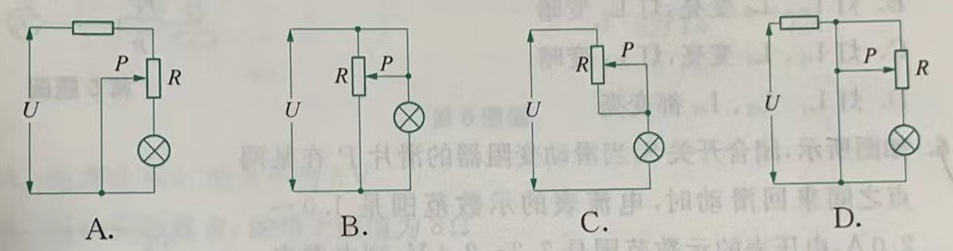
\includegraphics [scale=0.6,trim=0 0 0 0]{./image/physics_circuit3_1.png}
            % \caption{例1图}
            \label{fig:fig_circuit3_1}
        \end{figure}
        \vspace{2.5cm}

        \question[5] 在如图所示的电路中,$AB$为粗细均匀的长为$L$的电阻丝,以$AB$上各点对$B$点的电压$U$为纵坐标,
        各点距$A$点的距离为横坐标,则$U$随$x$变化的图线应为(\quad\quad\quad)。
        \begin{figure}[htb]
            \flushright
            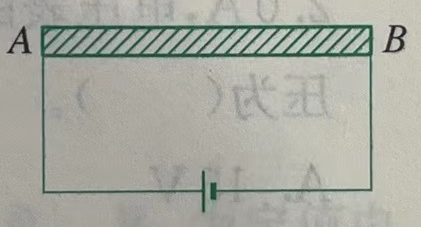
\includegraphics [scale=0.3,trim=0 0 0 0]{./image/physics_circuit3_2_1.png}
            % \caption{例1图}
            \label{fig:fig_circuit3_2_1}
        \end{figure}
        \begin{figure}[htb]
            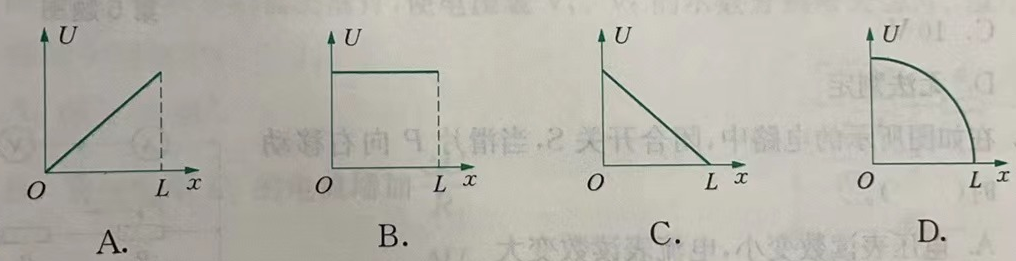
\includegraphics [scale=0.6,trim=0 0 0 0]{./image/physics_circuit3_2_2.png}
            % \caption{例1图}
            \label{fig:fig_circuit3_2_2}
        \end{figure}
        \vspace{2.5cm}

        \question[5] 如图所示,$R_1=20\Omega$,$R_2=25\Omega$,当开关$S_1$闭合、$S_2$断开时,电压表的示数为$2.8V$,
        当开关$S_1$断开、$S_2$闭合时,电压表示数可能的数值是(\quad\quad\quad)。
        \fourchoices{$4.0V$}
        {$3.5V$}
        {$3.3V$}
        {$2.5V$}
        \begin{figure}[htb]
            \flushright
            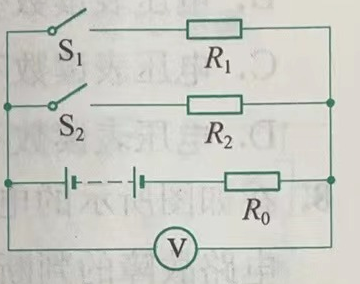
\includegraphics [scale=0.5,trim=0 0 0 0]{./image/physics_circuit3_3.png}
            % \caption{例1图}
            \label{fig:fig_circuit3_3}
        \end{figure}
        \vspace{2.5cm}

        \question[5] 在如图所示的电路中,电源电压为$4.5V$,且保持不变,电阻$R_1$的阻值为$5\Omega$,变阻器$R_2$的最大阻值为$20\Omega$,
        电流表的量程为$0\~{}0.6A$,电压表的量程为$0\~{}3V$。为保护电表,变阻器接入电路的阻值范围是(\quad\quad\quad)。
        \fourchoices{$2.5\~{}10\Omega$}
        {$0\~{}20\Omega$}
        {$2.5\~{}20\Omega$}
        {$0\~{}10\Omega$}
        \begin{figure}[htb]
            \flushright
            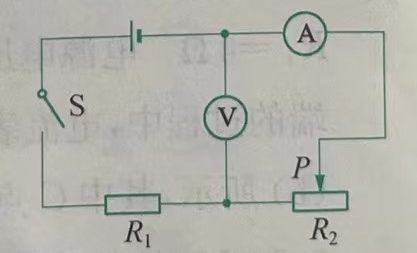
\includegraphics [scale=0.5,trim=0 0 0 0]{./image/physics_circuit3_4.png}
            % \caption{例1图}
            \label{fig:fig_circuit3_4}
        \end{figure}
        \vspace{3.5cm}

        \question[5] 在如图所示的电路中,电源电压保持不变,当闭合开关$S$后,将滑动变阻器的滑片向左滑动时(\quad\quad\quad)。
        \fourchoices{灯$L_1$、$L_3$变亮,灯$L_2$变暗}
        {灯$L_1$、$L_2$变亮,灯$L_3$变暗}
        {灯$L_2$、$L_3$变亮,灯$L_1$变暗}
        {灯$L_1$、$L_2$、$L_3$都变亮}
        \begin{figure}[htb]
            \flushright
            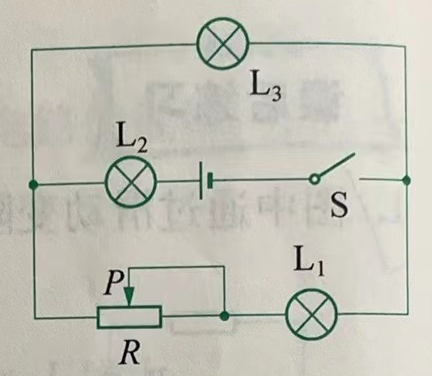
\includegraphics [scale=0.4,trim=0 0 0 0]{./image/physics_circuit3_5.png}
            % \caption{例1图}
            \label{fig:fig_circuit3_5}
        \end{figure}
        \vspace{2.5cm}

        \question[5] 如图所示,闭合开关$S$,当滑动变阻器的滑片$P$在某两点之间来回滑动时,
        电流表的示数范围是$1.0\~{}2.0A$,电压表的示数范围是$7.2\~{}2.4V$,则电源电压沩(\quad\quad\quad)。
        \fourchoices{$15V$}
        {$12V$}
        {$10V$}
        {无法确定}
        \begin{figure}[htb]
            \flushright
            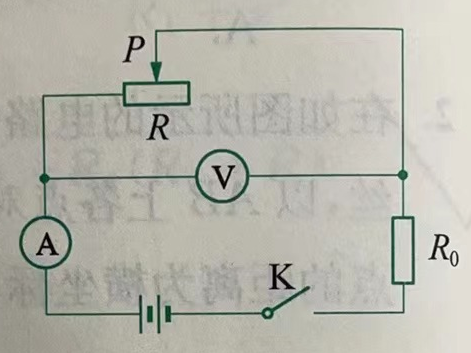
\includegraphics [scale=0.4,trim=0 0 0 0]{./image/physics_circuit3_6.png}
            % \caption{例1图}
            \label{fig:fig_circuit3_6}
        \end{figure}
        \vspace{2.5cm}

        \question[5] (多选)在如图所示的电路中,电源电压$U$保持不变,$R_1$、$R_2$、$R_3$为定值电阻,移动滑动变阻器的滑片,
        使电压表$V_1$、$V_2$的示数分别增大$\Delta U_1$、$\Delta U_2$,在这个过程中(\quad\quad\quad)。
        \fourchoices{$\Delta U_2<\Delta U_1$}
        {通过电阻$R_1$的电流增加$\frac{\Delta U_1}{R_1}$}
        {通过电阻$R_2$的电流减小$\frac{\Delta U_2}{R_3}$}
        {电阻$R_3$两端电压增大$\Delta U_2$}
        \begin{figure}[htb]
            \flushright
            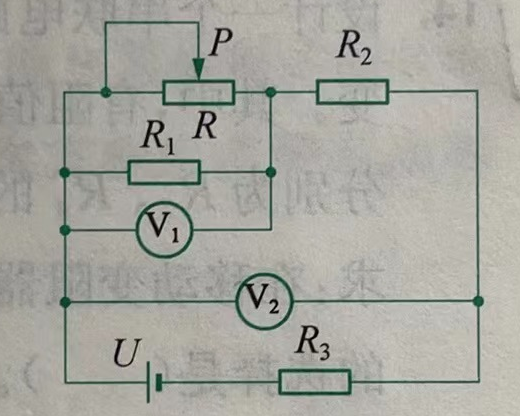
\includegraphics [scale=0.4,trim=0 0 0 0]{./image/physics_circuit3_7.png}
            % \caption{例1图}
            \label{fig:fig_circuit3_7}
        \end{figure}
        \vspace{2.5cm}

        \question[5] 在如图所示的电路中,无论电路中的电阻如何变化,设定流入电路的总电流始终保持恒定。当变阻器$R_0$
        的滑动触头向上滑动时,电压表$V$、电流表$A$的示数变化量分别为$\Delta U$、$\Delta I$,
        则$\left| \frac{\Delta U}{\Delta I} \right|$为(\quad\quad\quad)。
        \fourchoices{$R_1$}{$R_2$}{$R_1+R_2$}{$R_1-R_2$}
        \begin{figure}[htb]
            \flushright
            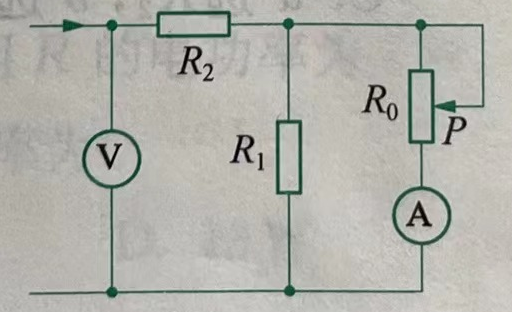
\includegraphics [scale=0.4,trim=0 0 0 0]{./image/physics_circuit3_8.png}
            % \caption{例1图}
            \label{fig:fig_circuit3_8}
        \end{figure}
        \vspace{2.5cm}

        \question[5] 某同学做电学实验,改变滑动变阻器接人电路的电阻大小,并测量记录了多组电压表和电流表的示数,
        根据数据分析,连接的电路可能是下面电路中的(\quad\quad\quad)。
        \begin{figure}[htb]
            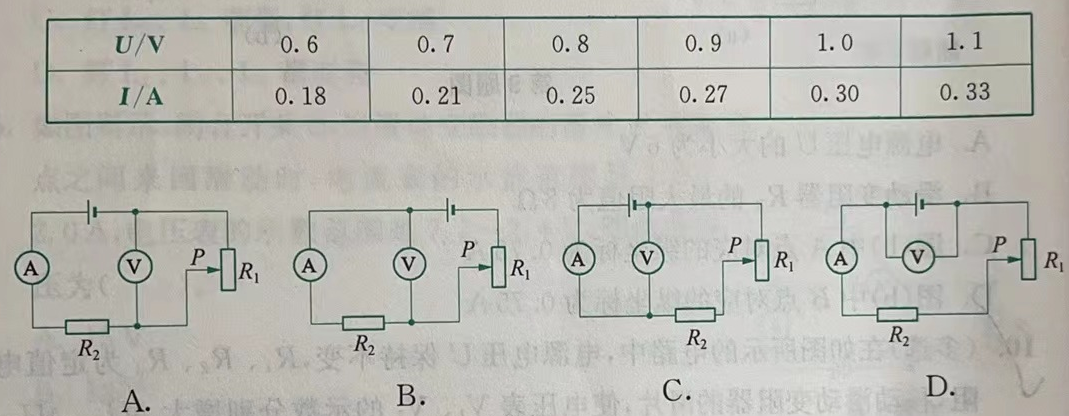
\includegraphics [scale=0.5,trim=0 0 0 0]{./image/physics_circuit3_9.png}
            % \caption{例1图}
            \label{fig:fig_circuit3_9}
        \end{figure}
        \vspace{2.5cm}

        \question[5] 设计一个串联电路,$a$表示定值电阻,$b$表示滑动变阻器,电源电压保持不变。
        其中,有阻值分别为$R_1$、$R_2$的两个定值电阻可供$a$选择,有最大阻值分别为$R_3$、$R_4$的两个滑动变阻器
        可供$b$选择,且$R_1<R_2<R_3<R_4$。要求:在移动变阻器滑片$P$的过程中,串联电路的电流变化范围最大,(\quad\quad\quad)。
        \fourchoices{$a$选$R_1$,$b$选$R_4$}
        {$a$选$R_1$,$b$选$R_3$}
        {$a$选$R_2$,$b$选$R_3$}
        {$a$选$R_2$,$b$选$R_4$}
        \vspace{2.5cm}

        \newpage
        
        \question[5] 如图所示,电源电压$U$不变,$R_0$、$R_1$均为定值电阻,滑动变阻器的最大阻值为$R$,
        在变阻器滑片$P$由$b$端缓慢滑到$a$端的过程中,试求:
        \begin{subquestions}
            \subquestion $A$、$B$ 两点间的电阻$R_{AB}$的变化情况。
            \subquestion 电流表 $A$、$A_1$、$A_2$示数的变化情况。
        \end{subquestions}
        \begin{figure}[htb]
            \flushright
            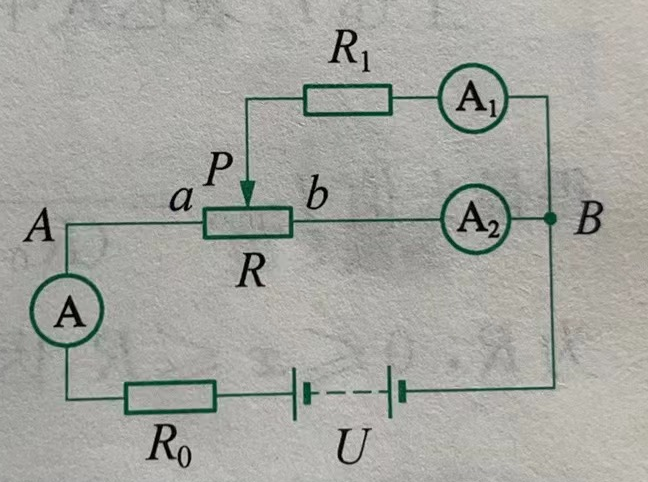
\includegraphics [scale=0.4,trim=0 0 0 0]{./image/physics_circuit3_10.png}
            % \caption{例1图}
            \label{fig:fig_circuit3_10}
        \end{figure}







    \end{questions}





\end{groups}


\label{lastpage}
\end{document}
